\chapter{Example benchmark code}

In this appendix, we consider the Python implementation of the GAT benchmark case -- both using Ein and NumPy. The case is based on an open-source implementation (in \href{https://github.com/google-deepmind/clrs/blob/8697f51663bd77548f4b3108816c84d163883361/clrs/_src/processors.py#L99}{\texttt{deepmind/clrs}} on GitHub) of Graph Attention Networks which used JAX, and which I translated by hand.

The excerpts from the implementations omit the surrounding test harness -- all free variables should be assumed to be function arguments, and imports (such as \mintinline{python}{from ein import array}) are presumed.

\section*{Ein}

\begin{minted}{python}
def softmax(x: Vec[T]) -> Vec[T]:
    x_max = fold_max(lambda i: x[i])
    x1 = array(lambda i: (x[i] - x_max).exp())
    x1_sum = fold_sum(lambda i: x1[i])
    return array(lambda i: x1[i] / x1_sum)
def leaky_relu(x: Scalar) -> Scalar:
    return where(x < 0.0, 0.01 * x, x)
bias = array(lambda b, u, v: (adj[b, u, v] - 1.0) * 1e9)
logits = array(lambda b, h, u, v: s[b, u, h] + t[b, v, h] + e[b, u, v, h] + g[b, h])
coefs = array(
    lambda b, h, u: softmax(array(lambda v: leaky_relu(logits[b, h, u, v]) + bias[b, u, v]))
)
return array(lambda b, u, h, f: fold_sum(lambda v: coefs[b, h, u, v] * vals[b, v, h, f]))
\end{minted}

\section*{NumPy}

\begin{minted}{python}
batches, vertices, heads = s.shape
bias = (adj - 1.0) * 1e9
bias = numpy.tile(bias[..., None], (1, 1, 1, heads))  # [B, N, N, H]
bias = numpy.transpose(bias, (0, 3, 1, 2))  # [B, H, N, N]
vals = numpy.transpose(vals, (0, 2, 1, 3))  # [B, H, N, F]
logits = (
    numpy.transpose(s[..., numpy.newaxis], (0, 2, 1, 3))  # + [B, H, N, 1]
    + numpy.transpose(t[..., numpy.newaxis], (0, 2, 3, 1))  # + [B, H, 1, N]
    + numpy.transpose(e, (0, 3, 1, 2))  # + [B, H, N, N]
    + g[..., numpy.newaxis, numpy.newaxis]  # + [B, H, 1, 1]
)  # = [B, H, N, N]
coefs = scipy.special.softmax(leaky_relu(logits) + bias, axis=-1)
ret = numpy.matmul(coefs, vals)  # [B, H, N, F]
return numpy.transpose(ret, (0, 2, 1, 3))  # [B, N, H, F]
\end{minted}

\chapter{Benchmark results}

This appendix provides extended benchmark results generated across many problem sizes, depicting any evident uncertainties and overheads associated with Ein. This solidifies arguments that Ein's performance is consistently at an satisfactory (though not perfectly optimal) level. 

This data further includes performance measurements for Ein's alternative backends -- PyTorch and JAX -- on cases based on deep learning domain programs. We did not consider this when evaluating Ein itself, as these backends have characteristics entirely independent from NumPy, hence comparisons to NumPy baselines would be unfair. Since JAX applies ahead-of-time compilation, it performs best of all.


\pgfplotsset{width=0.46\textwidth}
\begin{center}
% This file was created with tikzplotlib v0.10.1.
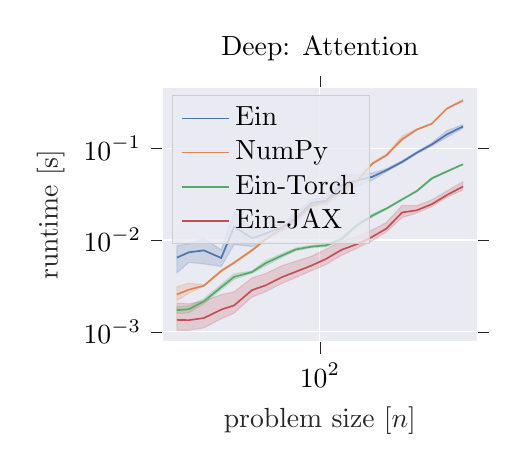
\begin{tikzpicture}

\definecolor{darkslategray38}{RGB}{38,38,38}
\definecolor{indianred1967882}{RGB}{196,78,82}
\definecolor{lavender234234242}{RGB}{234,234,242}
\definecolor{lightgray204}{RGB}{204,204,204}
\definecolor{mediumseagreen85168104}{RGB}{85,168,104}
\definecolor{peru22113282}{RGB}{221,132,82}
\definecolor{steelblue76114176}{RGB}{76,114,176}

\begin{axis}[
axis background/.style={fill=lavender234234242},
axis line style={white},
legend cell align={left},
legend style={
  fill opacity=0.8,
  draw opacity=1,
  text opacity=1,
  at={(0.03,0.97)},
  anchor=north west,
  draw=lightgray204,
  fill=lavender234234242
},
log basis x={10},
log basis y={10},
tick align=outside,
title={Deep: Attention},
x grid style={white},
xlabel=\textcolor{darkslategray38}{problem size \(\displaystyle [n]\)},
xmajorgrids,
xmajorticks=true,
xmin=46.6516495768404, xmax=214.354692507259,
xmode=log,
xtick style={color=darkslategray38},
xtick={1,10,100,1000,10000},
xticklabels={
  \(\displaystyle {10^{0}}\),
  \(\displaystyle {10^{1}}\),
  \(\displaystyle {10^{2}}\),
  \(\displaystyle {10^{3}}\),
  \(\displaystyle {10^{4}}\)
},
y grid style={white},
ylabel=\textcolor{darkslategray38}{runtime \(\displaystyle [\mathrm{s}]\)},
ymajorgrids,
ymajorticks=true,
ymin=0.00077839036959817, ymax=0.457526748594189,
ymode=log,
ytick style={color=darkslategray38},
ytick={1e-05,0.0001,0.001,0.01,0.1,1,10},
yticklabels={
  \(\displaystyle {10^{-5}}\),
  \(\displaystyle {10^{-4}}\),
  \(\displaystyle {10^{-3}}\),
  \(\displaystyle {10^{-2}}\),
  \(\displaystyle {10^{-1}}\),
  \(\displaystyle {10^{0}}\),
  \(\displaystyle {10^{1}}\)
}
]
\path [draw=steelblue76114176, fill=steelblue76114176, opacity=0.2]
(axis cs:50,0.00866516961777961)
--(axis cs:50,0.00437959733370008)
--(axis cs:53,0.00571136703130833)
--(axis cs:57,0.00549411397931181)
--(axis cs:62,0.00515819448823095)
--(axis cs:66,0.00892478528103311)
--(axis cs:72,0.00848875309562573)
--(axis cs:77,0.0103497280768715)
--(axis cs:83,0.0123574961470513)
--(axis cs:89,0.0153537073681036)
--(axis cs:96,0.0232318204215153)
--(axis cs:103,0.0243470966342829)
--(axis cs:111,0.0315116077092898)
--(axis cs:120,0.0389474992522446)
--(axis cs:129,0.0450581238989071)
--(axis cs:138,0.0553997155387656)
--(axis cs:149,0.0689141282858084)
--(axis cs:160,0.0869645879760659)
--(axis cs:172,0.105726904223739)
--(axis cs:185,0.131048314404507)
--(axis cs:200,0.165113660536008)
--(axis cs:200,0.180641041833345)
--(axis cs:200,0.180641041833345)
--(axis cs:185,0.155048844173325)
--(axis cs:172,0.114410946255666)
--(axis cs:160,0.0916533128799529)
--(axis cs:149,0.0734081268089115)
--(axis cs:138,0.0597020637572213)
--(axis cs:129,0.0539203415942211)
--(axis cs:120,0.0511957639434513)
--(axis cs:111,0.0529041254961703)
--(axis cs:103,0.0293612358650353)
--(axis cs:96,0.0277204202753455)
--(axis cs:89,0.019608219791935)
--(axis cs:83,0.0151259833710719)
--(axis cs:77,0.013628377620571)
--(axis cs:72,0.0132266213948424)
--(axis cs:66,0.020198493437565)
--(axis cs:62,0.007824812572253)
--(axis cs:57,0.0104621480692003)
--(axis cs:53,0.00908270323507167)
--(axis cs:50,0.00866516961777961)
--cycle;

\path [draw=peru22113282, fill=peru22113282, opacity=0.2]
(axis cs:50,0.00310353585159311)
--(axis cs:50,0.00218444558344713)
--(axis cs:53,0.00264099351667625)
--(axis cs:57,0.00312796367951597)
--(axis cs:62,0.00448941067160709)
--(axis cs:66,0.00557242847517711)
--(axis cs:72,0.00755672795249632)
--(axis cs:77,0.0100570621815171)
--(axis cs:83,0.0130532579372449)
--(axis cs:89,0.0164422829610364)
--(axis cs:96,0.0233506864421977)
--(axis cs:103,0.0257494977775032)
--(axis cs:111,0.033438777893418)
--(axis cs:120,0.0445056615972135)
--(axis cs:129,0.0666900751281689)
--(axis cs:138,0.0820565367084694)
--(axis cs:149,0.120457840584569)
--(axis cs:160,0.158036874815908)
--(axis cs:172,0.183906026934872)
--(axis cs:185,0.268949629911049)
--(axis cs:200,0.323277702575238)
--(axis cs:200,0.342407206869608)
--(axis cs:200,0.342407206869608)
--(axis cs:185,0.270939681069608)
--(axis cs:172,0.184995948976445)
--(axis cs:160,0.161979947460587)
--(axis cs:149,0.135785860485587)
--(axis cs:138,0.0860758318697544)
--(axis cs:129,0.0703926157974764)
--(axis cs:120,0.044865218588711)
--(axis cs:111,0.0359047128432406)
--(axis cs:103,0.0261409336381674)
--(axis cs:96,0.02392734355242)
--(axis cs:89,0.0167713351898807)
--(axis cs:83,0.0135379774516235)
--(axis cs:77,0.0103985540208683)
--(axis cs:72,0.00795292652835976)
--(axis cs:66,0.0057852893105983)
--(axis cs:62,0.00471289860325527)
--(axis cs:57,0.00324922433031861)
--(axis cs:53,0.00338942967117329)
--(axis cs:50,0.00310353585159311)
--cycle;

\path [draw=mediumseagreen85168104, fill=mediumseagreen85168104, opacity=0.2]
(axis cs:50,0.00187290531822601)
--(axis cs:50,0.00158513726851878)
--(axis cs:53,0.0016137860001219)
--(axis cs:57,0.00201893411013274)
--(axis cs:62,0.00289776546878525)
--(axis cs:66,0.00373102859269551)
--(axis cs:72,0.0043638359677626)
--(axis cs:77,0.00526634859471565)
--(axis cs:83,0.00644555344442868)
--(axis cs:89,0.00762556502617976)
--(axis cs:96,0.00826393439470511)
--(axis cs:103,0.00844199800456072)
--(axis cs:111,0.00998340065959914)
--(axis cs:120,0.0142332090726544)
--(axis cs:129,0.0178838018784524)
--(axis cs:138,0.0216053634271237)
--(axis cs:149,0.0273835782945794)
--(axis cs:160,0.0335230086783611)
--(axis cs:172,0.0457188929081333)
--(axis cs:185,0.055095821991904)
--(axis cs:200,0.0664708835104172)
--(axis cs:200,0.0671842281804)
--(axis cs:200,0.0671842281804)
--(axis cs:185,0.056459320917976)
--(axis cs:172,0.0479695519078791)
--(axis cs:160,0.0349625464752244)
--(axis cs:149,0.0280033654203467)
--(axis cs:138,0.0224041123807414)
--(axis cs:129,0.0192028373828745)
--(axis cs:120,0.0151070856808665)
--(axis cs:111,0.0105863185380748)
--(axis cs:103,0.00903352225843227)
--(axis cs:96,0.00872550573906673)
--(axis cs:89,0.00820928155905056)
--(axis cs:83,0.0070573557732735)
--(axis cs:77,0.00598837103111767)
--(axis cs:72,0.00462060092172372)
--(axis cs:66,0.00429114082115338)
--(axis cs:62,0.00328256745105565)
--(axis cs:57,0.00228848670919722)
--(axis cs:53,0.00191788660218393)
--(axis cs:50,0.00187290531822601)
--cycle;

\path [draw=indianred1967882, fill=indianred1967882, opacity=0.2]
(axis cs:50,0.00205881323224707)
--(axis cs:50,0.00104124689899113)
--(axis cs:53,0.0010400903012386)
--(axis cs:57,0.00110539173312424)
--(axis cs:62,0.00138889518446576)
--(axis cs:66,0.0016029928755513)
--(axis cs:72,0.00239549333605125)
--(axis cs:77,0.00274089793460654)
--(axis cs:83,0.003342213045646)
--(axis cs:89,0.00390773333814443)
--(axis cs:96,0.00463540845530101)
--(axis cs:103,0.00541510976137866)
--(axis cs:111,0.00678948703619883)
--(axis cs:120,0.00820162525218169)
--(axis cs:129,0.00984654562840018)
--(axis cs:138,0.0122467687309224)
--(axis cs:149,0.0175595193414461)
--(axis cs:160,0.0197309056472951)
--(axis cs:172,0.0231411516457184)
--(axis cs:185,0.0292151280773551)
--(axis cs:200,0.0351284628291287)
--(axis cs:200,0.0431678517648125)
--(axis cs:200,0.0431678517648125)
--(axis cs:185,0.0341627500656422)
--(axis cs:172,0.027380149367324)
--(axis cs:160,0.0237241203101732)
--(axis cs:149,0.0237959453089162)
--(axis cs:138,0.0155229372777814)
--(axis cs:129,0.0129405168089087)
--(axis cs:120,0.0108386296032014)
--(axis cs:111,0.0097959206418152)
--(axis cs:103,0.00792431511245824)
--(axis cs:96,0.00665502165672111)
--(axis cs:89,0.00588912678058672)
--(axis cs:83,0.0052340604459715)
--(axis cs:77,0.00432033834046546)
--(axis cs:72,0.00386931112517196)
--(axis cs:66,0.00272614762906446)
--(axis cs:62,0.00254660686450554)
--(axis cs:57,0.0021701492825976)
--(axis cs:53,0.00202190131528866)
--(axis cs:50,0.00205881323224707)
--cycle;

\addplot [semithick, steelblue76114176]
table {%
50 0.00643274999965797
53 0.00735101454993128
57 0.00771308540133759
62 0.00637658750201808
66 0.0140010272487416
72 0.0104482082519098
77 0.0118259001006663
83 0.0136795625010564
89 0.0172192685517075
96 0.0253301624994492
103 0.0267429874998925
111 0.0393433604527672
120 0.0446574875495571
129 0.0488993959479558
138 0.0575560601129028
149 0.0709554693312384
160 0.0894417500858253
172 0.109759966698766
185 0.141206109501582
200 0.172337763833639
};
\addlegendentry{Ein}
\addplot [semithick, peru22113282]
table {%
50 0.00255128515533029
53 0.0028795089613461
57 0.00318148329340343
62 0.00460141695582579
66 0.00566110787079768
72 0.00774117495072384
77 0.0102194417204102
83 0.0132789852982531
89 0.0165945225562473
96 0.0236534559910623
103 0.025940232301479
111 0.0343576448007313
120 0.0446880515076771
129 0.067997123383816
138 0.0837056615370571
149 0.125628829068229
160 0.159758864971689
172 0.184506074572662
185 0.269923098852367
200 0.32982686899833
};
\addlegendentry{NumPy}
\addplot [semithick, mediumseagreen85168104]
table {%
50 0.00172237945965705
53 0.00176415987976747
57 0.00214939264385376
62 0.00307004820947768
66 0.00397105576327044
72 0.00449107211043373
77 0.00561494950886657
83 0.00673614917752436
89 0.00790025604297564
96 0.00848050888403911
103 0.0087393636749908
111 0.0102517985659017
120 0.0146336277735162
129 0.0184530670706201
138 0.0219870518770367
149 0.0276830294999428
160 0.0341652543630178
172 0.0469080397933075
185 0.0557453297948299
200 0.0668298867097816
};
\addlegendentry{Ein-Torch}
\addplot [semithick, indianred1967882]
table {%
50 0.00134965422105551
53 0.0013415680448473
57 0.00141344694199765
62 0.00174696667797057
66 0.00194345548314172
72 0.00285092328542987
77 0.0032179174217509
83 0.00392467615481708
89 0.0045173176434051
96 0.00527181917109779
103 0.00622426011225447
111 0.00781238090470423
120 0.00906573866683564
129 0.0108542434016427
138 0.0133068508364409
149 0.0199720156130728
160 0.0210991645836497
172 0.0245697380430599
185 0.0309027223601388
200 0.0382407308824617
};
\addlegendentry{Ein-JAX}
\end{axis}

\end{tikzpicture}

% This file was created with tikzplotlib v0.10.1.
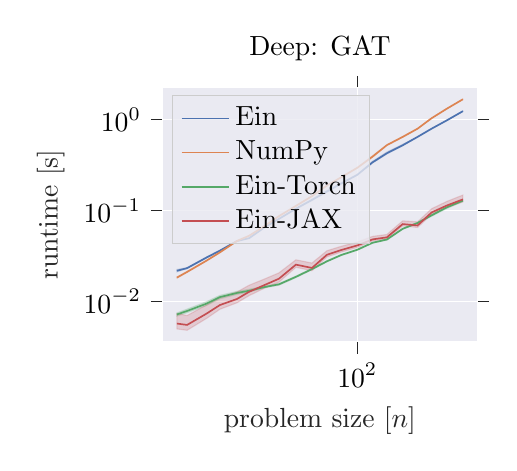
\begin{tikzpicture}

\definecolor{darkslategray38}{RGB}{38,38,38}
\definecolor{indianred1967882}{RGB}{196,78,82}
\definecolor{lavender234234242}{RGB}{234,234,242}
\definecolor{lightgray204}{RGB}{204,204,204}
\definecolor{mediumseagreen85168104}{RGB}{85,168,104}
\definecolor{peru22113282}{RGB}{221,132,82}
\definecolor{steelblue76114176}{RGB}{76,114,176}

\begin{axis}[
axis background/.style={fill=lavender234234242},
axis line style={white},
legend cell align={left},
legend style={
  fill opacity=0.8,
  draw opacity=1,
  text opacity=1,
  at={(0.03,0.97)},
  anchor=north west,
  draw=lightgray204,
  fill=lavender234234242
},
log basis x={10},
log basis y={10},
tick align=outside,
title={Deep: GAT},
x grid style={white},
xlabel=\textcolor{darkslategray38}{problem size \(\displaystyle [n]\)},
xmajorgrids,
xmajorticks=true,
xmin=47.327541132008, xmax=158.470096282431,
xmode=log,
xtick style={color=darkslategray38},
xtick={1,10,100,1000,10000},
xticklabels={
  \(\displaystyle {10^{0}}\),
  \(\displaystyle {10^{1}}\),
  \(\displaystyle {10^{2}}\),
  \(\displaystyle {10^{3}}\),
  \(\displaystyle {10^{4}}\)
},
y grid style={white},
ylabel=\textcolor{darkslategray38}{runtime \(\displaystyle [\mathrm{s}]\)},
ymajorgrids,
ymajorticks=true,
ymin=0.00357140451188423, ymax=2.26106159776395,
ymode=log,
ytick style={color=darkslategray38},
ytick={0.0001,0.001,0.01,0.1,1,10,100},
yticklabels={
  \(\displaystyle {10^{-4}}\),
  \(\displaystyle {10^{-3}}\),
  \(\displaystyle {10^{-2}}\),
  \(\displaystyle {10^{-1}}\),
  \(\displaystyle {10^{0}}\),
  \(\displaystyle {10^{1}}\),
  \(\displaystyle {10^{2}}\)
}
]
\path [draw=steelblue76114176, fill=steelblue76114176, opacity=0.2]
(axis cs:50,0.0224064104077843)
--(axis cs:50,0.0210412454555808)
--(axis cs:52,0.0229158697547246)
--(axis cs:56,0.0299149832124385)
--(axis cs:59,0.0358376364599826)
--(axis cs:63,0.0456729108822037)
--(axis cs:66,0.0491684852679646)
--(axis cs:70,0.0646785691614014)
--(axis cs:74,0.0803627570432022)
--(axis cs:79,0.103316506038318)
--(axis cs:84,0.128890981930363)
--(axis cs:89,0.159859436452669)
--(axis cs:94,0.195611296211367)
--(axis cs:100,0.246378408599412)
--(axis cs:106,0.333690374798607)
--(axis cs:112,0.41918990839913)
--(axis cs:119,0.516446224800893)
--(axis cs:126,0.64382335820701)
--(axis cs:133,0.794372391194338)
--(axis cs:141,0.981472824997036)
--(axis cs:150,1.23903302499966)
--(axis cs:150,1.24767705000122)
--(axis cs:150,1.24767705000122)
--(axis cs:141,0.987544958601939)
--(axis cs:133,0.800509074598085)
--(axis cs:126,0.64970140819787)
--(axis cs:119,0.534673908003606)
--(axis cs:112,0.440913625000394)
--(axis cs:106,0.348489816399524)
--(axis cs:100,0.249056608401588)
--(axis cs:94,0.203338528161112)
--(axis cs:89,0.166099075831049)
--(axis cs:84,0.133873198001311)
--(axis cs:79,0.106884058438336)
--(axis cs:74,0.0812587877306774)
--(axis cs:70,0.0657299229210821)
--(axis cs:66,0.0501189256020007)
--(axis cs:63,0.0465664724373346)
--(axis cs:59,0.0365034048300004)
--(axis cs:56,0.0306932388946916)
--(axis cs:52,0.0234602749724218)
--(axis cs:50,0.0224064104077843)
--cycle;

\path [draw=peru22113282, fill=peru22113282, opacity=0.2]
(axis cs:50,0.0184446637488246)
--(axis cs:50,0.0180389303494724)
--(axis cs:52,0.0208063706469779)
--(axis cs:56,0.027785318992844)
--(axis cs:59,0.0343131169008965)
--(axis cs:63,0.0460556466785556)
--(axis cs:66,0.0523332022301264)
--(axis cs:70,0.0669414899752905)
--(axis cs:74,0.0859334319641273)
--(axis cs:79,0.111642439610493)
--(axis cs:84,0.143552917215477)
--(axis cs:89,0.187321973106492)
--(axis cs:94,0.231179429897902)
--(axis cs:100,0.293751603926884)
--(axis cs:106,0.386191019495534)
--(axis cs:112,0.523593463389857)
--(axis cs:119,0.640901830344275)
--(axis cs:126,0.794109153360786)
--(axis cs:133,1.03776265251244)
--(axis cs:141,1.32023781367195)
--(axis cs:150,1.67623644593477)
--(axis cs:150,1.68644699609881)
--(axis cs:150,1.68644699609881)
--(axis cs:141,1.32596844847007)
--(axis cs:133,1.04090713381635)
--(axis cs:126,0.799377051096404)
--(axis cs:119,0.653990563834111)
--(axis cs:112,0.526348537227738)
--(axis cs:106,0.401894903748126)
--(axis cs:100,0.297173655463371)
--(axis cs:94,0.233740213749402)
--(axis cs:89,0.190098517411969)
--(axis cs:84,0.144045956168409)
--(axis cs:79,0.11321181335858)
--(axis cs:74,0.0877056620071769)
--(axis cs:70,0.0677325927020697)
--(axis cs:66,0.0530688906948059)
--(axis cs:63,0.0464273294289722)
--(axis cs:59,0.0348896895115116)
--(axis cs:56,0.0281341879859182)
--(axis cs:52,0.0213262885845254)
--(axis cs:50,0.0184446637488246)
--cycle;

\path [draw=mediumseagreen85168104, fill=mediumseagreen85168104, opacity=0.2]
(axis cs:50,0.00743295871048535)
--(axis cs:50,0.00687200388019871)
--(axis cs:52,0.0074930098752942)
--(axis cs:56,0.00897587326713843)
--(axis cs:59,0.0106428847682784)
--(axis cs:63,0.0119085282911349)
--(axis cs:66,0.0126129485285033)
--(axis cs:70,0.0140595800550794)
--(axis cs:74,0.0150293664085469)
--(axis cs:79,0.0182432389176254)
--(axis cs:84,0.0222616800430254)
--(axis cs:89,0.0272269726960217)
--(axis cs:94,0.0319773777120358)
--(axis cs:100,0.0365829273842013)
--(axis cs:106,0.0436282533725329)
--(axis cs:112,0.047242670973237)
--(axis cs:119,0.0621273175736479)
--(axis cs:126,0.0719567266462061)
--(axis cs:133,0.0865027543115848)
--(axis cs:141,0.105024522007452)
--(axis cs:150,0.126176274210953)
--(axis cs:150,0.130420841712754)
--(axis cs:150,0.130420841712754)
--(axis cs:141,0.113464524100065)
--(axis cs:133,0.0904368666775504)
--(axis cs:126,0.073952481209692)
--(axis cs:119,0.0634411171924257)
--(axis cs:112,0.0485145711111044)
--(axis cs:106,0.0446024222239718)
--(axis cs:100,0.0373581716624065)
--(axis cs:94,0.0326587859305207)
--(axis cs:89,0.0279756185996088)
--(axis cs:84,0.0230142008905059)
--(axis cs:79,0.0189408876615551)
--(axis cs:74,0.0156786140643163)
--(axis cs:70,0.0146691434408907)
--(axis cs:66,0.0135612458835837)
--(axis cs:63,0.0128472674165502)
--(axis cs:59,0.0116173681917336)
--(axis cs:56,0.00988141689946825)
--(axis cs:52,0.00818949443835985)
--(axis cs:50,0.00743295871048535)
--cycle;

\path [draw=indianred1967882, fill=indianred1967882, opacity=0.2]
(axis cs:50,0.00731889193440033)
--(axis cs:50,0.00495874899108899)
--(axis cs:52,0.00478827120602207)
--(axis cs:56,0.00644950759050617)
--(axis cs:59,0.00816689320752591)
--(axis cs:63,0.00962187027855653)
--(axis cs:66,0.0115327729351214)
--(axis cs:70,0.0139326398565619)
--(axis cs:74,0.0162365970744979)
--(axis cs:79,0.0236683298817417)
--(axis cs:84,0.0216872680642368)
--(axis cs:89,0.0308136652889306)
--(axis cs:94,0.0348492028240012)
--(axis cs:100,0.0392587054763064)
--(axis cs:106,0.0461627059877419)
--(axis cs:112,0.0487399533457126)
--(axis cs:119,0.0676435583134491)
--(axis cs:126,0.0650237155558534)
--(axis cs:133,0.0905544287291479)
--(axis cs:141,0.107433061663371)
--(axis cs:150,0.124204772754486)
--(axis cs:150,0.147991329348705)
--(axis cs:150,0.147991329348705)
--(axis cs:141,0.125908877168537)
--(axis cs:133,0.104513053144372)
--(axis cs:126,0.0749493139939688)
--(axis cs:119,0.0768664639600017)
--(axis cs:112,0.0544041973221155)
--(axis cs:106,0.0518374017672409)
--(axis cs:100,0.0449336621239608)
--(axis cs:94,0.0403161100861066)
--(axis cs:89,0.0360645335703938)
--(axis cs:84,0.0263720795233649)
--(axis cs:79,0.0286191008722177)
--(axis cs:74,0.0205508808193658)
--(axis cs:70,0.0175855829868509)
--(axis cs:66,0.0150278903494274)
--(axis cs:63,0.0126684991309)
--(axis cs:59,0.0110030724841527)
--(axis cs:56,0.00908455295077054)
--(axis cs:52,0.00696318723015097)
--(axis cs:50,0.00731889193440033)
--cycle;

\addplot [semithick, steelblue76114176]
table {%
50 0.0216760998991958
52 0.0231662792510178
56 0.0302682354493299
59 0.0361598061506811
63 0.0460759415494977
66 0.0495460314006777
70 0.0651565495018076
74 0.0808198366900727
79 0.104625850000593
84 0.130679302250428
89 0.16215188114854
94 0.198401333494985
100 0.247568916800083
106 0.33913195799978
112 0.427241775000584
119 0.523064891403192
126 0.64678057480196
133 0.79727589119575
141 0.984185700197122
150 1.2426766582008
};
\addlegendentry{Ein}
\addplot [semithick, peru22113282]
table {%
50 0.0182130364523043
52 0.0210364735598855
56 0.0279562927596381
59 0.03460015871306
63 0.0462338385518484
66 0.0526965015366717
70 0.0673173190473749
74 0.0866866368311044
79 0.112365184951298
84 0.143799225384102
89 0.188661039833064
94 0.232386050729092
100 0.295726299667496
106 0.392010738506597
112 0.524969192960174
119 0.646691693017161
126 0.796551988781993
133 1.03934860479822
141 1.32297764797611
150 1.68100227928949
};
\addlegendentry{NumPy}
\addplot [semithick, mediumseagreen85168104]
table {%
50 0.00715292066259177
52 0.00781948498840287
56 0.00939947963225524
59 0.0111208254302579
63 0.0123486733880478
66 0.0130629380760076
70 0.0143331227714161
74 0.015357040848465
79 0.0185846830770869
84 0.0226133333008199
89 0.0275805378776561
94 0.032319371216476
100 0.0369736208737475
106 0.0441079508953219
112 0.0478854620460647
119 0.0628114840339826
126 0.0729227797616792
133 0.0884276606554327
141 0.108415097274186
150 0.12845207085672
};
\addlegendentry{Ein-Torch}
\addplot [semithick, indianred1967882]
table {%
50 0.00568068419057727
52 0.0054860035885484
56 0.00729115811799732
59 0.00909071010385364
63 0.0106026201235609
66 0.0127219582809245
70 0.0150839495721233
74 0.0177233758812232
79 0.0253218013106487
84 0.0232849760647165
89 0.0325735358667949
94 0.0366899236671074
100 0.0412307227256109
106 0.0480314079229481
112 0.0506300543985476
119 0.0708419455383009
126 0.0684180482507702
133 0.0951441087412742
141 0.113442764289238
150 0.132628757479829
};
\addlegendentry{Ein-JAX}
\end{axis}

\end{tikzpicture}

\end{center}
\begin{center}
% This file was created with tikzplotlib v0.10.1.
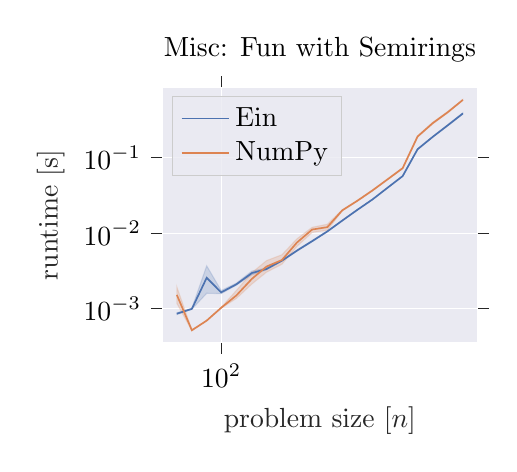
\begin{tikzpicture}

\definecolor{darkslategray38}{RGB}{38,38,38}
\definecolor{lavender234234242}{RGB}{234,234,242}
\definecolor{lightgray204}{RGB}{204,204,204}
\definecolor{peru22113282}{RGB}{221,132,82}
\definecolor{steelblue76114176}{RGB}{76,114,176}

\begin{axis}[
axis background/.style={fill=lavender234234242},
axis line style={white},
legend cell align={left},
legend style={
  fill opacity=0.8,
  draw opacity=1,
  text opacity=1,
  at={(0.03,0.97)},
  anchor=north west,
  draw=lightgray204,
  fill=lavender234234242
},
log basis x={10},
log basis y={10},
tick align=outside,
title={Misc: Fun with Semirings},
x grid style={white},
xlabel=\textcolor{darkslategray38}{problem size \(\displaystyle [n]\)},
xmajorgrids,
xmajorticks=true,
xmin=62.3875656693622, xmax=785.412918011374,
xmode=log,
xtick style={color=darkslategray38},
xtick={1,10,100,1000,10000},
xticklabels={
  \(\displaystyle {10^{0}}\),
  \(\displaystyle {10^{1}}\),
  \(\displaystyle {10^{2}}\),
  \(\displaystyle {10^{3}}\),
  \(\displaystyle {10^{4}}\)
},
y grid style={white},
ylabel=\textcolor{darkslategray38}{runtime \(\displaystyle [\mathrm{s}]\)},
ymajorgrids,
ymajorticks=true,
ymin=0.000360273084941951, ymax=0.840756866074562,
ymode=log,
ytick style={color=darkslategray38},
ytick={1e-05,0.0001,0.001,0.01,0.1,1,10},
yticklabels={
  \(\displaystyle {10^{-5}}\),
  \(\displaystyle {10^{-4}}\),
  \(\displaystyle {10^{-3}}\),
  \(\displaystyle {10^{-2}}\),
  \(\displaystyle {10^{-1}}\),
  \(\displaystyle {10^{0}}\),
  \(\displaystyle {10^{1}}\)
}
]
\path [draw=steelblue76114176, fill=steelblue76114176, opacity=0.2]
(axis cs:70,0.000882980736569152)
--(axis cs:70,0.000836469603709702)
--(axis cs:79,0.000983666491465556)
--(axis cs:89,0.00160017079695535)
--(axis cs:100,0.00158288053147771)
--(axis cs:113,0.00204948378828703)
--(axis cs:128,0.00280844490238451)
--(axis cs:144,0.00326712702590157)
--(axis cs:163,0.00426672655372386)
--(axis cs:184,0.00577486806374509)
--(axis cs:208,0.00770885239919153)
--(axis cs:235,0.0104360073216048)
--(axis cs:265,0.0145424592601194)
--(axis cs:299,0.0201871005468638)
--(axis cs:338,0.0277885871910621)
--(axis cs:381,0.0395295096395785)
--(axis cs:431,0.0567088302808366)
--(axis cs:486,0.127795878605548)
--(axis cs:549,0.187310844089916)
--(axis cs:620,0.264747474796604)
--(axis cs:700,0.379321700398577)
--(axis cs:700,0.392475692002336)
--(axis cs:700,0.392475692002336)
--(axis cs:620,0.273306374798995)
--(axis cs:549,0.190437548428054)
--(axis cs:486,0.131277720707976)
--(axis cs:431,0.0574690455018653)
--(axis cs:381,0.0400586240080884)
--(axis cs:338,0.0281631004092378)
--(axis cs:299,0.0204711578140632)
--(axis cs:265,0.0148268214958807)
--(axis cs:235,0.0106902608964265)
--(axis cs:208,0.00799688121056533)
--(axis cs:184,0.00599107745618312)
--(axis cs:163,0.0043952521038409)
--(axis cs:144,0.00346288692931921)
--(axis cs:128,0.00314344688005804)
--(axis cs:113,0.00217874632706298)
--(axis cs:100,0.00173873103536607)
--(axis cs:89,0.00369602308688627)
--(axis cs:79,0.00101039469656826)
--(axis cs:70,0.000882980736569152)
--cycle;

\path [draw=peru22113282, fill=peru22113282, opacity=0.2]
(axis cs:70,0.00193848101255118)
--(axis cs:70,0.00117677244190284)
--(axis cs:79,0.000512536126241976)
--(axis cs:89,0.000691374327275463)
--(axis cs:100,0.00101480922461673)
--(axis cs:113,0.0013658054360003)
--(axis cs:128,0.00212054063949876)
--(axis cs:144,0.00304233388874813)
--(axis cs:163,0.00387155986232424)
--(axis cs:184,0.00667547516394288)
--(axis cs:208,0.0102306443561746)
--(axis cs:235,0.0109339212095422)
--(axis cs:265,0.019764288904906)
--(axis cs:299,0.0264826368818243)
--(axis cs:338,0.0363230633929786)
--(axis cs:381,0.0508596943735536)
--(axis cs:431,0.0714440472078674)
--(axis cs:486,0.187855203689419)
--(axis cs:549,0.280232980105275)
--(axis cs:620,0.393550276078777)
--(axis cs:700,0.577770442721567)
--(axis cs:700,0.590986770138042)
--(axis cs:700,0.590986770138042)
--(axis cs:620,0.408690926201109)
--(axis cs:549,0.293886953764823)
--(axis cs:486,0.194362045148285)
--(axis cs:431,0.0738519055358364)
--(axis cs:381,0.0519194425429355)
--(axis cs:338,0.0373699798928444)
--(axis cs:299,0.0271283243346789)
--(axis cs:265,0.020363228674962)
--(axis cs:235,0.0131407148729523)
--(axis cs:208,0.0119519829952601)
--(axis cs:184,0.00840683975339437)
--(axis cs:163,0.00517817608230361)
--(axis cs:144,0.00432445873980756)
--(axis cs:128,0.00299782580115713)
--(axis cs:113,0.00174265249451506)
--(axis cs:100,0.00104073359240367)
--(axis cs:89,0.000698650182437273)
--(axis cs:79,0.000523782635826371)
--(axis cs:70,0.00193848101255118)
--cycle;

\addplot [semithick, steelblue76114176]
table {%
70 0.000857760399958352
79 0.000994293649273459
89 0.00256512295018183
100 0.00164436434788513
113 0.00210113954890403
128 0.00296312304708408
144 0.00335419795010239
163 0.00432160414857208
184 0.00587280215040664
208 0.0078401249491435
235 0.0105500666497392
265 0.0146726103506808
299 0.0203304040995135
338 0.027970593853388
381 0.0397933979991649
431 0.0570397616684204
486 0.129457755250769
549 0.188722222330398
620 0.269026924797799
700 0.38559165839979
};
\addlegendentry{Ein}
\addplot [semithick, peru22113282]
table {%
70 0.00152205276548332
79 0.000517646586514327
89 0.000694967112294748
100 0.00102787029947846
113 0.00149808545271352
128 0.00247987456241484
144 0.00361289884685628
163 0.00440781469366663
184 0.00751455303028802
208 0.0111746290230265
235 0.0120248630362191
265 0.020062592361727
299 0.0268113644896092
338 0.0368154788839337
381 0.0513946486001272
431 0.0726436004298779
486 0.190808159953479
549 0.286831809215619
620 0.401049157632001
700 0.583262162683683
};
\addlegendentry{NumPy}
\end{axis}

\end{tikzpicture}

% This file was created with tikzplotlib v0.10.1.
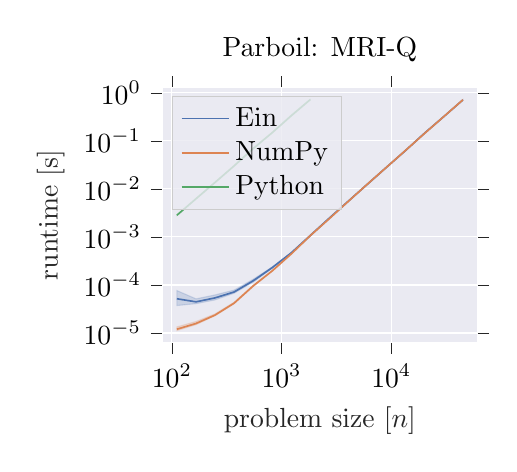
\begin{tikzpicture}

\definecolor{darkslategray38}{RGB}{38,38,38}
\definecolor{lavender234234242}{RGB}{234,234,242}
\definecolor{lightgray204}{RGB}{204,204,204}
\definecolor{mediumseagreen85168104}{RGB}{85,168,104}
\definecolor{peru22113282}{RGB}{221,132,82}
\definecolor{steelblue76114176}{RGB}{76,114,176}

\begin{axis}[
axis background/.style={fill=lavender234234242},
axis line style={white},
legend cell align={left},
legend style={
  fill opacity=0.8,
  draw opacity=1,
  text opacity=1,
  at={(0.03,0.97)},
  anchor=north west,
  draw=lightgray204,
  fill=lavender234234242
},
log basis x={10},
log basis y={10},
tick align=outside,
title={Parboil: MRI-Q},
x grid style={white},
xlabel=\textcolor{darkslategray38}{problem size \(\displaystyle [n]\)},
xmajorgrids,
xmajorticks=true,
xmin=82.2173119053552, xmax=60656.4224057923,
xmode=log,
xtick style={color=darkslategray38},
xtick={1,10,100,1000,10000,100000,1000000},
xticklabels={
  \(\displaystyle {10^{0}}\),
  \(\displaystyle {10^{1}}\),
  \(\displaystyle {10^{2}}\),
  \(\displaystyle {10^{3}}\),
  \(\displaystyle {10^{4}}\),
  \(\displaystyle {10^{5}}\),
  \(\displaystyle {10^{6}}\)
},
y grid style={white},
ylabel=\textcolor{darkslategray38}{runtime \(\displaystyle [\mathrm{s}]\)},
ymajorgrids,
ymajorticks=true,
ymin=6.44509514937527e-06, ymax=1.27001142277489,
ymode=log,
ytick style={color=darkslategray38},
ytick={1e-07,1e-06,1e-05,0.0001,0.001,0.01,0.1,1,10,100},
yticklabels={
  \(\displaystyle {10^{-7}}\),
  \(\displaystyle {10^{-6}}\),
  \(\displaystyle {10^{-5}}\),
  \(\displaystyle {10^{-4}}\),
  \(\displaystyle {10^{-3}}\),
  \(\displaystyle {10^{-2}}\),
  \(\displaystyle {10^{-1}}\),
  \(\displaystyle {10^{0}}\),
  \(\displaystyle {10^{1}}\),
  \(\displaystyle {10^{2}}\)
}
]
\path [draw=steelblue76114176, fill=steelblue76114176, opacity=0.2]
(axis cs:111,7.64748115580005e-05)
--(axis cs:111,3.72972208060673e-05)
--(axis cs:166,4.0835252875695e-05)
--(axis cs:247,4.88473840596271e-05)
--(axis cs:369,6.7268329221406e-05)
--(axis cs:551,0.000114852847618749)
--(axis cs:822,0.000223653940593067)
--(axis cs:1227,0.000462866237739945)
--(axis cs:1830,0.00106242175335865)
--(axis cs:2731,0.00245355305976773)
--(axis cs:4074,0.00557270789158792)
--(axis cs:6078,0.0125523086427165)
--(axis cs:9069,0.0283365872718605)
--(axis cs:13530,0.0632754475533375)
--(axis cs:20185,0.145936900787482)
--(axis cs:30115,0.320605041601812)
--(axis cs:44928,0.712623358200653)
--(axis cs:44928,0.714020192003227)
--(axis cs:44928,0.714020192003227)
--(axis cs:30115,0.321693008599686)
--(axis cs:20185,0.14665374558499)
--(axis cs:13530,0.0637399425110971)
--(axis cs:9069,0.0285860408108601)
--(axis cs:6078,0.0127089362215156)
--(axis cs:4074,0.00564107549882465)
--(axis cs:2731,0.00251207519948366)
--(axis cs:1830,0.00109240443509407)
--(axis cs:1227,0.000473713477222191)
--(axis cs:822,0.000237093156229093)
--(axis cs:551,0.000131444422586355)
--(axis cs:369,7.81547400038107e-05)
--(axis cs:247,6.19402840311523e-05)
--(axis cs:166,5.13782398957119e-05)
--(axis cs:111,7.64748115580005e-05)
--cycle;

\path [draw=peru22113282, fill=peru22113282, opacity=0.2]
(axis cs:111,1.33739018919205e-05)
--(axis cs:111,1.12173942238236e-05)
--(axis cs:166,1.49132007232064e-05)
--(axis cs:247,2.28202668057949e-05)
--(axis cs:369,4.062789333185e-05)
--(axis cs:551,9.28342900732395e-05)
--(axis cs:822,0.000195022538156002)
--(axis cs:1227,0.000440077011060149)
--(axis cs:1830,0.00105853735348736)
--(axis cs:2731,0.00240892100099761)
--(axis cs:4074,0.00553731830009614)
--(axis cs:6078,0.012528845465293)
--(axis cs:9069,0.0282633957795509)
--(axis cs:13530,0.0633936064423404)
--(axis cs:20185,0.143992453522449)
--(axis cs:30115,0.32144269773129)
--(axis cs:44928,0.713192287989754)
--(axis cs:44928,0.720010642417622)
--(axis cs:44928,0.720010642417622)
--(axis cs:30115,0.322048080552488)
--(axis cs:20185,0.144803723048071)
--(axis cs:13530,0.0644441558384659)
--(axis cs:9069,0.0286264725029522)
--(axis cs:6078,0.0128897941919057)
--(axis cs:4074,0.00559594220218362)
--(axis cs:2731,0.00242732959793209)
--(axis cs:1830,0.00108295461147436)
--(axis cs:1227,0.000450903698156903)
--(axis cs:822,0.000199314085446513)
--(axis cs:551,9.87969676543967e-05)
--(axis cs:369,4.36825888719407e-05)
--(axis cs:247,2.49443589484715e-05)
--(axis cs:166,1.73521935363702e-05)
--(axis cs:111,1.33739018919205e-05)
--cycle;

\path [draw=mediumseagreen85168104, fill=mediumseagreen85168104, opacity=0.2]
(axis cs:111,0.00284139199984255)
--(axis cs:111,0.00281315856921844)
--(axis cs:166,0.00620528220835487)
--(axis cs:247,0.0135245814389517)
--(axis cs:369,0.0300064772016471)
--(axis cs:551,0.0690009891442962)
--(axis cs:822,0.148020185515479)
--(axis cs:1227,0.328925585642)
--(axis cs:1830,0.727446436590146)
--(axis cs:1830,0.729701060447134)
--(axis cs:1830,0.729701060447134)
--(axis cs:1227,0.346346094633531)
--(axis cs:822,0.14927478996866)
--(axis cs:551,0.0694211350693412)
--(axis cs:369,0.0302894853075574)
--(axis cs:247,0.0136903077843667)
--(axis cs:166,0.00628679223794377)
--(axis cs:111,0.00284139199984255)
--cycle;

\addplot [semithick, steelblue76114176]
table {%
111 5.16250009241048e-05
166 4.45396020950284e-05
247 5.37770007213112e-05
369 7.14415997208562e-05
551 0.00012215835013194
822 0.000229739699716447
1227 0.000467931201274041
1830 0.00107539789896691
2731 0.00248072924878215
4074 0.00560521049992531
6078 0.0126218833531311
9069 0.0284476669010473
13530 0.0635063490017274
20185 0.146266012140716
30115 0.321243258399772
44928 0.713352350203786
};
\addlegendentry{Ein}
\addplot [semithick, peru22113282]
table {%
111 1.19852447942259e-05
166 1.57818105550113e-05
247 2.35852213674601e-05
369 4.17824449198122e-05
551 9.55665661751828e-05
822 0.000196775694192413
1227 0.000445184290021028
1830 0.00107005975987052
2731 0.00241792426754517
4074 0.00556451805312463
6078 0.0126745723357563
9069 0.0284252734792757
13530 0.0638591521675768
20185 0.144395721890358
30115 0.321745246758947
44928 0.716419132342862
};
\addlegendentry{NumPy}
\addplot [semithick, mediumseagreen85168104]
table {%
111 0.00282732900447953
166 0.00624331846538919
247 0.0136108447615918
369 0.0301533647669631
551 0.0692055784849342
822 0.148659283175515
1227 0.335733234812183
1830 0.728610696513374
};
\addlegendentry{Python}
\end{axis}

\end{tikzpicture}

\end{center}
\begin{center}
% This file was created with tikzplotlib v0.10.1.
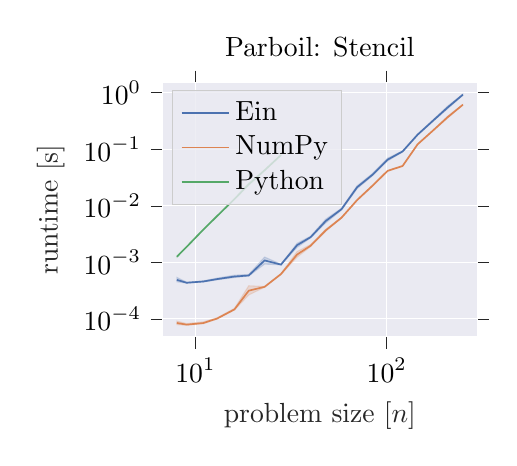
\begin{tikzpicture}

\definecolor{darkslategray38}{RGB}{38,38,38}
\definecolor{lavender234234242}{RGB}{234,234,242}
\definecolor{lightgray204}{RGB}{204,204,204}
\definecolor{mediumseagreen85168104}{RGB}{85,168,104}
\definecolor{peru22113282}{RGB}{221,132,82}
\definecolor{steelblue76114176}{RGB}{76,114,176}

\begin{axis}[
axis background/.style={fill=lavender234234242},
axis line style={white},
legend cell align={left},
legend style={
  fill opacity=0.8,
  draw opacity=1,
  text opacity=1,
  at={(0.03,0.97)},
  anchor=north west,
  draw=lightgray204,
  fill=lavender234234242
},
log basis x={10},
log basis y={10},
tick align=outside,
title={Parboil: Stencil},
x grid style={white},
xlabel=\textcolor{darkslategray38}{problem size \(\displaystyle [n]\)},
xmajorgrids,
xmajorticks=true,
xmin=6.73515331060639, xmax=296.949439421139,
xmode=log,
xtick style={color=darkslategray38},
xtick={0.1,1,10,100,1000,10000},
xticklabels={
  \(\displaystyle {10^{-1}}\),
  \(\displaystyle {10^{0}}\),
  \(\displaystyle {10^{1}}\),
  \(\displaystyle {10^{2}}\),
  \(\displaystyle {10^{3}}\),
  \(\displaystyle {10^{4}}\)
},
y grid style={white},
ylabel=\textcolor{darkslategray38}{runtime \(\displaystyle [\mathrm{s}]\)},
ymajorgrids,
ymajorticks=true,
ymin=4.83051032061226e-05, ymax=1.51304214299554,
ymode=log,
ytick style={color=darkslategray38},
ytick={1e-06,1e-05,0.0001,0.001,0.01,0.1,1,10,100},
yticklabels={
  \(\displaystyle {10^{-6}}\),
  \(\displaystyle {10^{-5}}\),
  \(\displaystyle {10^{-4}}\),
  \(\displaystyle {10^{-3}}\),
  \(\displaystyle {10^{-2}}\),
  \(\displaystyle {10^{-1}}\),
  \(\displaystyle {10^{0}}\),
  \(\displaystyle {10^{1}}\),
  \(\displaystyle {10^{2}}\)
}
]
\path [draw=steelblue76114176, fill=steelblue76114176, opacity=0.2]
(axis cs:8,0.000541935047749575)
--(axis cs:8,0.000453067858434224)
--(axis cs:9,0.000429355900341761)
--(axis cs:11,0.000449767605587112)
--(axis cs:13,0.000491204320896941)
--(axis cs:16,0.000538839243417897)
--(axis cs:19,0.000574791597191506)
--(axis cs:23,0.000931360130489338)
--(axis cs:28,0.000902584986779402)
--(axis cs:34,0.00184224452015769)
--(axis cs:40,0.00270429013589819)
--(axis cs:48,0.00497561136766308)
--(axis cs:58,0.0083633242857286)
--(axis cs:70,0.0200854641618207)
--(axis cs:84,0.0336955659928026)
--(axis cs:101,0.0620397576999039)
--(axis cs:121,0.0895633316013779)
--(axis cs:145,0.177699520667375)
--(axis cs:174,0.309677375195315)
--(axis cs:208,0.519359374797205)
--(axis cs:250,0.901571849806351)
--(axis cs:250,0.945134991791565)
--(axis cs:250,0.945134991791565)
--(axis cs:208,0.578511466801865)
--(axis cs:174,0.328275911873352)
--(axis cs:145,0.185667826333277)
--(axis cs:121,0.0935580004773576)
--(axis cs:101,0.0694506404745198)
--(axis cs:84,0.03691085733215)
--(axis cs:70,0.0226090456772181)
--(axis cs:58,0.00903003433808408)
--(axis cs:48,0.00581493507243067)
--(axis cs:40,0.00289911827871038)
--(axis cs:34,0.00217413936628873)
--(axis cs:28,0.00092799956431918)
--(axis cs:23,0.00124031511919384)
--(axis cs:19,0.000610801349448593)
--(axis cs:16,0.000592792265306343)
--(axis cs:13,0.000526802544554812)
--(axis cs:11,0.000469785337154463)
--(axis cs:9,0.000446724885805452)
--(axis cs:8,0.000541935047749575)
--cycle;

\path [draw=peru22113282, fill=peru22113282, opacity=0.2]
(axis cs:8,9.13596512038154e-05)
--(axis cs:8,7.91657086267016e-05)
--(axis cs:9,7.73303893172656e-05)
--(axis cs:11,8.21614088033308e-05)
--(axis cs:13,9.99987730910563e-05)
--(axis cs:16,0.000143655783890312)
--(axis cs:19,0.000264574498680686)
--(axis cs:23,0.000365250698994858)
--(axis cs:28,0.000610801170047995)
--(axis cs:34,0.00123471806723196)
--(axis cs:40,0.00189975958156038)
--(axis cs:48,0.00353642528071143)
--(axis cs:58,0.00606321318274284)
--(axis cs:70,0.0124189869511541)
--(axis cs:84,0.0219762063405069)
--(axis cs:101,0.0407717955827718)
--(axis cs:121,0.0498527350103243)
--(axis cs:145,0.120981924009612)
--(axis cs:174,0.210022050049381)
--(axis cs:208,0.355438718990264)
--(axis cs:250,0.609366626672306)
--(axis cs:250,0.61736012092859)
--(axis cs:250,0.61736012092859)
--(axis cs:208,0.38465304082684)
--(axis cs:174,0.215096195849646)
--(axis cs:145,0.123596176361213)
--(axis cs:121,0.0513678632191388)
--(axis cs:101,0.0420714220593185)
--(axis cs:84,0.023028867715002)
--(axis cs:70,0.0128413578502985)
--(axis cs:58,0.00625039350995157)
--(axis cs:48,0.0038478141557566)
--(axis cs:40,0.00206198302403562)
--(axis cs:34,0.0015508935681735)
--(axis cs:28,0.000631648145628399)
--(axis cs:23,0.000374060347589935)
--(axis cs:19,0.000385554545724589)
--(axis cs:16,0.000153494512630142)
--(axis cs:13,0.000104623943702111)
--(axis cs:11,8.87077325713449e-05)
--(axis cs:9,8.26492469642159e-05)
--(axis cs:8,9.13596512038154e-05)
--cycle;

\path [draw=mediumseagreen85168104, fill=mediumseagreen85168104, opacity=0.2]
(axis cs:8,0.0012659812533587)
--(axis cs:8,0.00124678293925191)
--(axis cs:9,0.00186972866893111)
--(axis cs:11,0.00375912878122672)
--(axis cs:13,0.00657057378940949)
--(axis cs:16,0.0130797217000369)
--(axis cs:19,0.0230161577127175)
--(axis cs:23,0.0422440562527591)
--(axis cs:28,0.078720046293707)
--(axis cs:28,0.0792059575627619)
--(axis cs:28,0.0792059575627619)
--(axis cs:23,0.0427538768824543)
--(axis cs:19,0.0252667824897221)
--(axis cs:16,0.0131840415997233)
--(axis cs:13,0.00665563404754166)
--(axis cs:11,0.00382769138591117)
--(axis cs:9,0.00188651765983936)
--(axis cs:8,0.0012659812533587)
--cycle;

\addplot [semithick, steelblue76114176]
table {%
8 0.000490091650135582
9 0.00043558534962358
11 0.000458699947921559
13 0.00050575009881868
16 0.000561285449657589
19 0.0005851313493622
23 0.00108082085134811
28 0.000912118700216524
34 0.00201392704766477
40 0.00278657515082159
48 0.00538161674849107
58 0.00869469794924953
70 0.0212869855029567
84 0.0351202103032847
101 0.0653614270631806
121 0.0913993370909752
145 0.181004548501126
174 0.316765899996972
208 0.546782341599464
250 0.923486833198695
};
\addlegendentry{Ein}
\addplot [semithick, peru22113282]
table {%
8 8.47601791404994e-05
9 7.91695351916375e-05
11 8.44630429538325e-05
13 0.000101679819065032
16 0.000147276848182292
19 0.000315438086191837
23 0.000368938222948831
28 0.000619920396183299
34 0.00137503175349805
40 0.00196653281810455
48 0.00368448892433253
58 0.00615190295006863
70 0.0126113480173802
84 0.0224496099670639
101 0.041402507229599
121 0.0505987697507714
145 0.122319606508964
174 0.212361871103318
208 0.368015794918882
250 0.613350352027503
};
\addlegendentry{NumPy}
\addplot [semithick, mediumseagreen85168104]
table {%
8 0.00125621954094339
9 0.00187764126625355
11 0.00379152600667076
13 0.00661218941234588
16 0.0131311919068916
19 0.023976585210625
23 0.0424380686665551
28 0.0789373184016279
};
\addlegendentry{Python}
\end{axis}

\end{tikzpicture}

% This file was created with tikzplotlib v0.10.1.
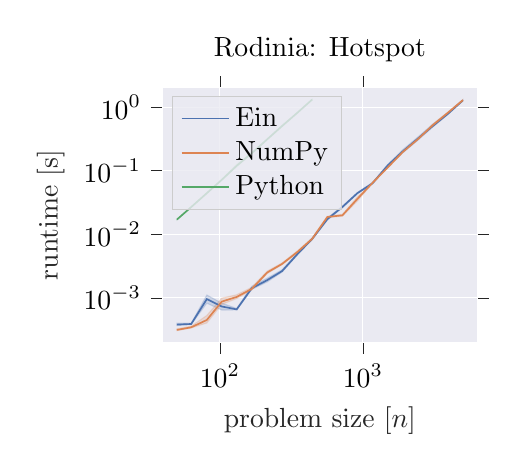
\begin{tikzpicture}

\definecolor{darkslategray38}{RGB}{38,38,38}
\definecolor{lavender234234242}{RGB}{234,234,242}
\definecolor{lightgray204}{RGB}{204,204,204}
\definecolor{mediumseagreen85168104}{RGB}{85,168,104}
\definecolor{peru22113282}{RGB}{221,132,82}
\definecolor{steelblue76114176}{RGB}{76,114,176}

\begin{axis}[
axis background/.style={fill=lavender234234242},
axis line style={white},
legend cell align={left},
legend style={
  fill opacity=0.8,
  draw opacity=1,
  text opacity=1,
  at={(0.03,0.97)},
  anchor=north west,
  draw=lightgray204,
  fill=lavender234234242
},
log basis x={10},
log basis y={10},
tick align=outside,
title={Rodinia: Hotspot},
x grid style={white},
xlabel=\textcolor{darkslategray38}{problem size \(\displaystyle [n]\)},
xmajorgrids,
xmajorticks=true,
xmin=39.7164117362141, xmax=6294.62705897084,
xmode=log,
xtick style={color=darkslategray38},
xtick={1,10,100,1000,10000,100000},
xticklabels={
  \(\displaystyle {10^{0}}\),
  \(\displaystyle {10^{1}}\),
  \(\displaystyle {10^{2}}\),
  \(\displaystyle {10^{3}}\),
  \(\displaystyle {10^{4}}\),
  \(\displaystyle {10^{5}}\)
},
y grid style={white},
ylabel=\textcolor{darkslategray38}{runtime \(\displaystyle [\mathrm{s}]\)},
ymajorgrids,
ymajorticks=true,
ymin=0.000201498092592216, ymax=2.00986678493088,
ymode=log,
ytick style={color=darkslategray38},
ytick={1e-05,0.0001,0.001,0.01,0.1,1,10,100},
yticklabels={
  \(\displaystyle {10^{-5}}\),
  \(\displaystyle {10^{-4}}\),
  \(\displaystyle {10^{-3}}\),
  \(\displaystyle {10^{-2}}\),
  \(\displaystyle {10^{-1}}\),
  \(\displaystyle {10^{0}}\),
  \(\displaystyle {10^{1}}\),
  \(\displaystyle {10^{2}}\)
}
]
\path [draw=steelblue76114176, fill=steelblue76114176, opacity=0.2]
(axis cs:50,0.00040093945186527)
--(axis cs:50,0.000368074528014404)
--(axis cs:63,0.000383445476672932)
--(axis cs:81,0.000825838538330572)
--(axis cs:103,0.000644772650684899)
--(axis cs:131,0.000647616701608058)
--(axis cs:167,0.00136470559069494)
--(axis cs:214,0.00178437005424712)
--(axis cs:272,0.00254733308358482)
--(axis cs:347,0.00471379582675581)
--(axis cs:442,0.00828688624365895)
--(axis cs:564,0.0167107987225791)
--(axis cs:719,0.0262008863759002)
--(axis cs:916,0.0437042131731141)
--(axis cs:1167,0.0622562896341378)
--(axis cs:1488,0.118060100646188)
--(axis cs:1896,0.190832166402834)
--(axis cs:2416,0.300329749798402)
--(axis cs:3079,0.486450566604617)
--(axis cs:3923,0.76613618300762)
--(axis cs:5000,1.26078589159588)
--(axis cs:5000,1.3012147084024)
--(axis cs:5000,1.3012147084024)
--(axis cs:3923,0.816607733399724)
--(axis cs:3079,0.541300269858912)
--(axis cs:2416,0.337273958601872)
--(axis cs:1896,0.213914475007914)
--(axis cs:1488,0.124943806214368)
--(axis cs:1167,0.0654436717586123)
--(axis cs:916,0.0455387166381115)
--(axis cs:719,0.0278046610032288)
--(axis cs:564,0.0180667039872242)
--(axis cs:442,0.00872899553934985)
--(axis cs:347,0.00499742749540019)
--(axis cs:272,0.00276927246466585)
--(axis cs:214,0.00204196582904842)
--(axis cs:167,0.00152384682147385)
--(axis cs:131,0.000682757289960136)
--(axis cs:103,0.000827624445300898)
--(axis cs:81,0.00111092252625895)
--(axis cs:63,0.000398907133476314)
--(axis cs:50,0.00040093945186527)
--cycle;

\path [draw=peru22113282, fill=peru22113282, opacity=0.2]
(axis cs:50,0.00032673171002542)
--(axis cs:50,0.000306223809256533)
--(axis cs:63,0.000337079613283184)
--(axis cs:81,0.000403104442021472)
--(axis cs:103,0.000791844439091519)
--(axis cs:131,0.000976233270458262)
--(axis cs:167,0.00133326872230646)
--(axis cs:214,0.00240886333381857)
--(axis cs:272,0.003335313129242)
--(axis cs:347,0.00508983559719171)
--(axis cs:442,0.00821648794715782)
--(axis cs:564,0.018363774495602)
--(axis cs:719,0.0192549980784647)
--(axis cs:916,0.0335724327249124)
--(axis cs:1167,0.0636838874629534)
--(axis cs:1488,0.110583235301932)
--(axis cs:1896,0.193861714741803)
--(axis cs:2416,0.306879325940162)
--(axis cs:3079,0.505523018210414)
--(axis cs:3923,0.799800217307046)
--(axis cs:5000,1.264736683983)
--(axis cs:5000,1.31620264555326)
--(axis cs:5000,1.31620264555326)
--(axis cs:3923,0.837685994555397)
--(axis cs:3079,0.539811122722255)
--(axis cs:2416,0.318958040986727)
--(axis cs:1896,0.199532320670354)
--(axis cs:1488,0.114055102252696)
--(axis cs:1167,0.0652174438192701)
--(axis cs:916,0.0388684300518635)
--(axis cs:719,0.0206627060913336)
--(axis cs:564,0.0192027732355738)
--(axis cs:442,0.00883587755718326)
--(axis cs:347,0.00546277709638322)
--(axis cs:272,0.00355156857035007)
--(axis cs:214,0.00263857985262473)
--(axis cs:167,0.00147028904430777)
--(axis cs:131,0.00112115848759694)
--(axis cs:103,0.000992268569379521)
--(axis cs:81,0.000529755718533716)
--(axis cs:63,0.000359117092669337)
--(axis cs:50,0.00032673171002542)
--cycle;

\path [draw=mediumseagreen85168104, fill=mediumseagreen85168104, opacity=0.2]
(axis cs:50,0.0171492615072016)
--(axis cs:50,0.0169266795758594)
--(axis cs:63,0.0266131099362991)
--(axis cs:81,0.0440128870918064)
--(axis cs:103,0.07126383819766)
--(axis cs:131,0.116134618129277)
--(axis cs:167,0.187049734661776)
--(axis cs:214,0.308844255432755)
--(axis cs:272,0.496620497434416)
--(axis cs:347,0.81118520515641)
--(axis cs:442,1.31659624124695)
--(axis cs:442,1.32251089329489)
--(axis cs:442,1.32251089329489)
--(axis cs:347,0.812763998462663)
--(axis cs:272,0.519172390597327)
--(axis cs:214,0.314748820935053)
--(axis cs:167,0.191087127589291)
--(axis cs:131,0.125872881631466)
--(axis cs:103,0.0727092836864279)
--(axis cs:81,0.0447864388573507)
--(axis cs:63,0.0270812682079353)
--(axis cs:50,0.0171492615072016)
--cycle;

\addplot [semithick, steelblue76114176]
table {%
50 0.000380316599330399
63 0.000389060348970816
81 0.000958352151792496
103 0.000733785350894323
131 0.000660091650934191
167 0.00141973749778117
214 0.00190174600284081
272 0.00264312924773549
347 0.00484016244954546
442 0.00849062289998983
564 0.0173506560495298
719 0.0269802436996542
916 0.04452330624772
1167 0.0634414349378858
1488 0.120880361001279
1896 0.200819791603135
2416 0.31828747499967
3079 0.505030508202617
3923 0.783784091603593
5000 1.28100029999914
};
\addlegendentry{Ein}
\addplot [semithick, peru22113282]
table {%
50 0.000313751671644151
63 0.00034511540423769
81 0.000449974981914862
103 0.000874762900493183
131 0.00103676393950919
167 0.00138504208322672
214 0.00250934550967851
272 0.00342247601949238
347 0.00524075549648738
442 0.00849938419192227
564 0.0187414299273627
719 0.0199229283698736
916 0.0362555841655364
1167 0.0644407811628573
1488 0.112207148416363
1896 0.196310843395679
2416 0.312149828431074
3079 0.521080107533942
3923 0.814798008302104
5000 1.28977514403189
};
\addlegendentry{NumPy}
\addplot [semithick, mediumseagreen85168104]
table {%
50 0.0170372362644735
63 0.0268527433421794
81 0.0444024117848814
103 0.0719782158874706
131 0.119667906225472
167 0.189060234167748
214 0.311685812135787
272 0.504449041617114
347 0.812088850100548
442 1.31957545728193
};
\addlegendentry{Python}
\end{axis}

\end{tikzpicture}

\end{center}
\begin{center}
% This file was created with tikzplotlib v0.10.1.
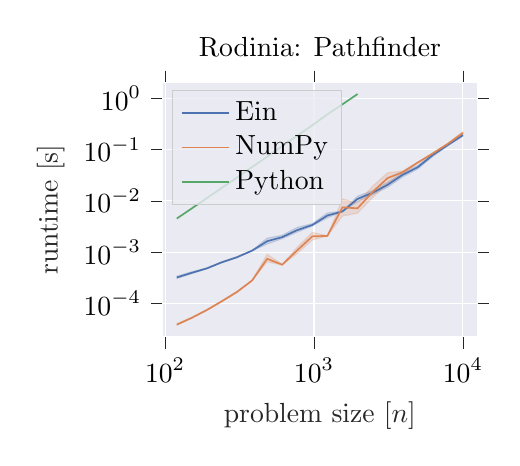
\begin{tikzpicture}

\definecolor{darkslategray38}{RGB}{38,38,38}
\definecolor{lavender234234242}{RGB}{234,234,242}
\definecolor{lightgray204}{RGB}{204,204,204}
\definecolor{mediumseagreen85168104}{RGB}{85,168,104}
\definecolor{peru22113282}{RGB}{221,132,82}
\definecolor{steelblue76114176}{RGB}{76,114,176}

\begin{axis}[
axis background/.style={fill=lavender234234242},
axis line style={white},
legend cell align={left},
legend style={
  fill opacity=0.8,
  draw opacity=1,
  text opacity=1,
  at={(0.03,0.97)},
  anchor=north west,
  draw=lightgray204,
  fill=lavender234234242
},
log basis x={10},
log basis y={10},
tick align=outside,
title={Rodinia: Pathfinder},
x grid style={white},
xlabel=\textcolor{darkslategray38}{problem size \(\displaystyle [n]\)},
xmajorgrids,
xmajorticks=true,
xmin=96.1922998493838, xmax=12475.0110131366,
xmode=log,
xtick style={color=darkslategray38},
xtick={1,10,100,1000,10000,100000,1000000},
xticklabels={
  \(\displaystyle {10^{0}}\),
  \(\displaystyle {10^{1}}\),
  \(\displaystyle {10^{2}}\),
  \(\displaystyle {10^{3}}\),
  \(\displaystyle {10^{4}}\),
  \(\displaystyle {10^{5}}\),
  \(\displaystyle {10^{6}}\)
},
y grid style={white},
ylabel=\textcolor{darkslategray38}{runtime \(\displaystyle [\mathrm{s}]\)},
ymajorgrids,
ymajorticks=true,
ymin=2.2418522596979e-05, ymax=2.02262511777973,
ymode=log,
ytick style={color=darkslategray38},
ytick={1e-06,1e-05,0.0001,0.001,0.01,0.1,1,10,100},
yticklabels={
  \(\displaystyle {10^{-6}}\),
  \(\displaystyle {10^{-5}}\),
  \(\displaystyle {10^{-4}}\),
  \(\displaystyle {10^{-3}}\),
  \(\displaystyle {10^{-2}}\),
  \(\displaystyle {10^{-1}}\),
  \(\displaystyle {10^{0}}\),
  \(\displaystyle {10^{1}}\),
  \(\displaystyle {10^{2}}\)
}
]
\path [draw=steelblue76114176, fill=steelblue76114176, opacity=0.2]
(axis cs:120,0.000341726930964796)
--(axis cs:120,0.000306472893898899)
--(axis cs:151,0.000380524324009457)
--(axis cs:191,0.000475164178642444)
--(axis cs:241,0.000622518288109859)
--(axis cs:304,0.000780791235338256)
--(axis cs:384,0.00105858095441363)
--(axis cs:485,0.0014339613285847)
--(axis cs:612,0.00182949863126851)
--(axis cs:772,0.00245332813254208)
--(axis cs:975,0.00322873239420005)
--(axis cs:1230,0.0046603400319691)
--(axis cs:1553,0.00614925598643822)
--(axis cs:1960,0.0095943368870212)
--(axis cs:2474,0.0131162009411673)
--(axis cs:3122,0.0184126407171061)
--(axis cs:3941,0.0291354026384579)
--(axis cs:4974,0.0417086751744864)
--(axis cs:6277,0.0726598048349842)
--(axis cs:7923,0.118049233426548)
--(axis cs:10000,0.1817131320034)
--(axis cs:10000,0.204999416671247)
--(axis cs:10000,0.204999416671247)
--(axis cs:7923,0.128127749075995)
--(axis cs:6277,0.083734567083649)
--(axis cs:4974,0.0490543335992334)
--(axis cs:3941,0.0353001864768157)
--(axis cs:3122,0.0230370064200542)
--(axis cs:2474,0.0158103541443779)
--(axis cs:1960,0.0123458300823404)
--(axis cs:1553,0.0063026045256629)
--(axis cs:1230,0.00581660559701049)
--(axis cs:975,0.00359588766476008)
--(axis cs:772,0.00303963665832271)
--(axis cs:612,0.00213747135527228)
--(axis cs:485,0.0018773853993298)
--(axis cs:384,0.00108018522152634)
--(axis cs:304,0.000818749898280657)
--(axis cs:241,0.000652531522373465)
--(axis cs:191,0.000493188765976811)
--(axis cs:151,0.000415084914093313)
--(axis cs:120,0.000341726930964796)
--cycle;

\path [draw=peru22113282, fill=peru22113282, opacity=0.2]
(axis cs:120,4.05292028394652e-05)
--(axis cs:120,3.76572221177818e-05)
--(axis cs:151,5.15489040017335e-05)
--(axis cs:191,7.37133692938077e-05)
--(axis cs:241,0.000108863147358759)
--(axis cs:304,0.00016458389057526)
--(axis cs:384,0.000277424925640168)
--(axis cs:485,0.000644754050045128)
--(axis cs:612,0.000561306121472983)
--(axis cs:772,0.000945457267077864)
--(axis cs:975,0.00171881254987961)
--(axis cs:1230,0.00206152069904944)
--(axis cs:1553,0.00504187347480254)
--(axis cs:1960,0.00572239232308683)
--(axis cs:2474,0.0115250413096875)
--(axis cs:3122,0.0217258990204398)
--(axis cs:3941,0.0334428679968257)
--(axis cs:4974,0.0548838507420711)
--(axis cs:6277,0.0824095292239567)
--(axis cs:7923,0.126775335965419)
--(axis cs:10000,0.201898616792484)
--(axis cs:10000,0.224101366947745)
--(axis cs:10000,0.224101366947745)
--(axis cs:7923,0.132007286081162)
--(axis cs:6277,0.0853363105666736)
--(axis cs:4974,0.0565887416299204)
--(axis cs:3941,0.0383505131565081)
--(axis cs:3122,0.03528248513181)
--(axis cs:2474,0.0192043702785523)
--(axis cs:1960,0.00920419509298448)
--(axis cs:1553,0.0108464514986388)
--(axis cs:1230,0.00208173524225237)
--(axis cs:975,0.0024281130370177)
--(axis cs:772,0.00124802802831195)
--(axis cs:612,0.00057954685688131)
--(axis cs:485,0.000910760384406102)
--(axis cs:384,0.000283834486956713)
--(axis cs:304,0.000172147029546981)
--(axis cs:241,0.00011356738586769)
--(axis cs:191,7.60678164252169e-05)
--(axis cs:151,5.38777557057058e-05)
--(axis cs:120,4.05292028394652e-05)
--cycle;

\path [draw=mediumseagreen85168104, fill=mediumseagreen85168104, opacity=0.2]
(axis cs:120,0.00455871063264353)
--(axis cs:120,0.00449157143116792)
--(axis cs:151,0.00705664282240553)
--(axis cs:191,0.0112666225017015)
--(axis cs:241,0.0179427403300778)
--(axis cs:304,0.0282595000777108)
--(axis cs:384,0.045413275318881)
--(axis cs:485,0.0720816022037464)
--(axis cs:612,0.115601016419376)
--(axis cs:772,0.18487746708988)
--(axis cs:975,0.293471200991418)
--(axis cs:1230,0.481217045161424)
--(axis cs:1553,0.755620449817535)
--(axis cs:1960,1.19882571494297)
--(axis cs:1960,1.2041320192535)
--(axis cs:1960,1.2041320192535)
--(axis cs:1553,0.766056252441126)
--(axis cs:1230,0.486687586993213)
--(axis cs:975,0.300764526207406)
--(axis cs:772,0.187704668997105)
--(axis cs:612,0.11655834188607)
--(axis cs:485,0.0725001043405431)
--(axis cs:384,0.0457697327409285)
--(axis cs:304,0.0284581307418256)
--(axis cs:241,0.0180423590589997)
--(axis cs:191,0.011370876864278)
--(axis cs:151,0.00713747732596371)
--(axis cs:120,0.00455871063264353)
--cycle;

\addplot [semithick, steelblue76114176]
table {%
120 0.000320914650365012
151 0.000395139447937254
191 0.000483020901447162
241 0.000635822951153386
304 0.000795981250121258
384 0.00106819585125777
485 0.0016338312496373
612 0.0019634500516986
772 0.00269066685068537
975 0.00338468330010073
1230 0.00516932915124926
1553 0.00620426465029595
1960 0.0108929021487711
2474 0.014341264700488
3122 0.0205118332502025
3941 0.0322111937006412
4974 0.0452253313495021
6277 0.0781504904600577
7923 0.122558375112324
10000 0.19009911116882
};
\addlegendentry{Ein}
\addplot [semithick, peru22113282]
table {%
120 3.86600244931162e-05
151 5.23924914005125e-05
191 7.46212748891676e-05
241 0.000110693301001573
304 0.000167543510974984
384 0.000279794247711953
485 0.000741863875427135
612 0.000569439187306788
772 0.00108637716541252
975 0.0020312529826725
1230 0.00207120530354192
1553 0.00746278985508761
1960 0.00712931676217431
2474 0.0148365315915019
3122 0.0277522884342686
3941 0.0361839926787512
4974 0.0557543046914908
6277 0.0839329969844282
7923 0.129218504613934
10000 0.210188051602755
};
\addlegendentry{NumPy}
\addplot [semithick, mediumseagreen85168104]
table {%
120 0.00452345369735408
151 0.00709796155077178
191 0.0113156319885714
241 0.0179928968837197
304 0.0283531498755143
384 0.0455828779890031
485 0.0722714566850368
612 0.116039105793265
772 0.186124559536344
975 0.296669488554691
1230 0.483990980228694
1553 0.759446551183138
1960 1.20162530253334
};
\addlegendentry{Python}
\end{axis}

\end{tikzpicture}

% This file was created with tikzplotlib v0.10.1.
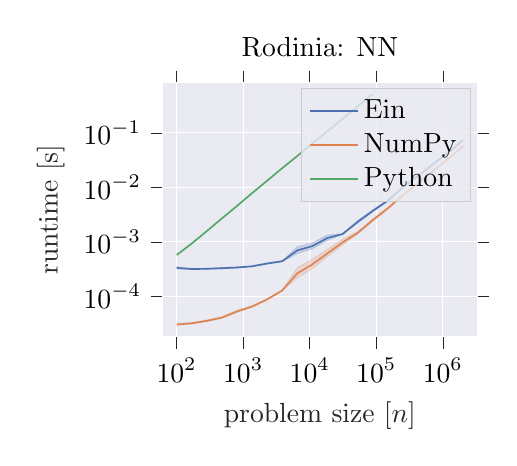
\begin{tikzpicture}

\definecolor{darkslategray38}{RGB}{38,38,38}
\definecolor{lavender234234242}{RGB}{234,234,242}
\definecolor{lightgray204}{RGB}{204,204,204}
\definecolor{mediumseagreen85168104}{RGB}{85,168,104}
\definecolor{peru22113282}{RGB}{221,132,82}
\definecolor{steelblue76114176}{RGB}{76,114,176}

\begin{axis}[
axis background/.style={fill=lavender234234242},
axis line style={white},
legend cell align={left},
legend style={
  fill opacity=0.8,
  draw opacity=1,
  text opacity=1,
  draw=lightgray204,
  fill=lavender234234242
},
log basis x={10},
log basis y={10},
tick align=outside,
title={Rodinia: NN},
x grid style={white},
xlabel=\textcolor{darkslategray38}{problem size \(\displaystyle [n]\)},
xmajorgrids,
xmajorticks=true,
xmin=61.5865594359247, xmax=3279936.43174958,
xmode=log,
xtick style={color=darkslategray38},
xtick={1,10,100,1000,10000,100000,1000000,10000000,100000000},
xticklabels={
  \(\displaystyle {10^{0}}\),
  \(\displaystyle {10^{1}}\),
  \(\displaystyle {10^{2}}\),
  \(\displaystyle {10^{3}}\),
  \(\displaystyle {10^{4}}\),
  \(\displaystyle {10^{5}}\),
  \(\displaystyle {10^{6}}\),
  \(\displaystyle {10^{7}}\),
  \(\displaystyle {10^{8}}\)
},
y grid style={white},
ylabel=\textcolor{darkslategray38}{runtime \(\displaystyle [\mathrm{s}]\)},
ymajorgrids,
ymajorticks=true,
ymin=1.81947944318841e-05, ymax=0.839521688084527,
ymode=log,
ytick style={color=darkslategray38},
ytick={1e-06,1e-05,0.0001,0.001,0.01,0.1,1,10},
yticklabels={
  \(\displaystyle {10^{-6}}\),
  \(\displaystyle {10^{-5}}\),
  \(\displaystyle {10^{-4}}\),
  \(\displaystyle {10^{-3}}\),
  \(\displaystyle {10^{-2}}\),
  \(\displaystyle {10^{-1}}\),
  \(\displaystyle {10^{0}}\),
  \(\displaystyle {10^{1}}\)
}
]
\path [draw=steelblue76114176, fill=steelblue76114176, opacity=0.2]
(axis cs:101,0.000353183350853215)
--(axis cs:101,0.000322000755368208)
--(axis cs:170,0.000314380267118395)
--(axis cs:286,0.000317003530926741)
--(axis cs:481,0.000322697213905485)
--(axis cs:810,0.000334883444993466)
--(axis cs:1364,0.000352830739120691)
--(axis cs:2297,0.000393298693052202)
--(axis cs:3866,0.000437682356459845)
--(axis cs:6508,0.000610060642447934)
--(axis cs:10954,0.000748529692882585)
--(axis cs:18439,0.00107022395513923)
--(axis cs:31037,0.0013778470563193)
--(axis cs:52243,0.00220267150323707)
--(axis cs:87937,0.00354220306126081)
--(axis cs:148018,0.00552566797723557)
--(axis cs:249149,0.00984000897233273)
--(axis cs:419374,0.0157586040781098)
--(axis cs:705902,0.0262687281757098)
--(axis cs:1188194,0.0427564917887139)
--(axis cs:2000000,0.0721616613371225)
--(axis cs:2000000,0.0738775504718173)
--(axis cs:2000000,0.0738775504718173)
--(axis cs:1188194,0.0434651341967401)
--(axis cs:705902,0.0266722735361873)
--(axis cs:419374,0.0162754852996295)
--(axis cs:249149,0.0101439765249415)
--(axis cs:148018,0.00586161805647862)
--(axis cs:87937,0.0038486267659755)
--(axis cs:52243,0.00245423619433495)
--(axis cs:31037,0.00140523523068623)
--(axis cs:18439,0.0013424137828224)
--(axis cs:10954,0.000953390890881565)
--(axis cs:6508,0.000815215431102843)
--(axis cs:3866,0.00044905472001119)
--(axis cs:2297,0.00040965498505102)
--(axis cs:1364,0.000361619109044113)
--(axis cs:810,0.000346027625691931)
--(axis cs:481,0.000339486644388671)
--(axis cs:286,0.000327328193470748)
--(axis cs:170,0.000322710332693532)
--(axis cs:101,0.000353183350853215)
--cycle;

\path [draw=peru22113282, fill=peru22113282, opacity=0.2]
(axis cs:101,3.22559100401596e-05)
--(axis cs:101,2.96449693902489e-05)
--(axis cs:170,3.14934114268439e-05)
--(axis cs:286,3.48214441480291e-05)
--(axis cs:481,4.00659476672678e-05)
--(axis cs:810,5.07766298240826e-05)
--(axis cs:1364,6.35731459038473e-05)
--(axis cs:2297,8.71387222680512e-05)
--(axis cs:3866,0.0001274504644238)
--(axis cs:6508,0.000219516355946705)
--(axis cs:10954,0.00032421837460516)
--(axis cs:18439,0.000541176797972362)
--(axis cs:31037,0.000875860084372431)
--(axis cs:52243,0.00139754218193783)
--(axis cs:87936.9999999999,0.00238507747289486)
--(axis cs:148018,0.00397239848397111)
--(axis cs:249149,0.00693343404896193)
--(axis cs:419374,0.011701289388949)
--(axis cs:705902,0.0196380316798663)
--(axis cs:1188194,0.0327551329863903)
--(axis cs:2000000,0.0563697438910666)
--(axis cs:2000000,0.0567656971331198)
--(axis cs:2000000,0.0567656971331198)
--(axis cs:1188194,0.0330266446635957)
--(axis cs:705902,0.020009598896486)
--(axis cs:419374,0.0121253361396363)
--(axis cs:249149,0.00723793720397841)
--(axis cs:148018,0.00425602114828713)
--(axis cs:87936.9999999999,0.00262417958025749)
--(axis cs:52243,0.00154237070974182)
--(axis cs:31037,0.00111702348559922)
--(axis cs:18439,0.000733776703379504)
--(axis cs:10954,0.000480482764834311)
--(axis cs:6508,0.000334941548718695)
--(axis cs:3866,0.000130604314644266)
--(axis cs:2297,9.00585693711033e-05)
--(axis cs:1364,6.78827531542254e-05)
--(axis cs:810,5.5947379509631e-05)
--(axis cs:481,4.22765473712785e-05)
--(axis cs:286,3.71984245268413e-05)
--(axis cs:170,3.31572100669677e-05)
--(axis cs:101,3.22559100401596e-05)
--cycle;

\path [draw=mediumseagreen85168104, fill=mediumseagreen85168104, opacity=0.2]
(axis cs:101,0.000589457024414009)
--(axis cs:101,0.000568953687788088)
--(axis cs:170,0.000932760601906098)
--(axis cs:286,0.00157676212682705)
--(axis cs:481,0.00269014023387063)
--(axis cs:810,0.00456824403507154)
--(axis cs:1364,0.00781684567576174)
--(axis cs:2297,0.0132332147399879)
--(axis cs:3866,0.0224030687894545)
--(axis cs:6508,0.0375410743138903)
--(axis cs:10954,0.0636976314951003)
--(axis cs:18439,0.106880695886844)
--(axis cs:31037,0.180381141286895)
--(axis cs:52243,0.302955803728834)
--(axis cs:87936.9999999999,0.513305702468478)
--(axis cs:87936.9999999999,0.515261943256742)
--(axis cs:87936.9999999999,0.515261943256742)
--(axis cs:52243,0.306912435547992)
--(axis cs:31037,0.181994994172091)
--(axis cs:18439,0.107544237911094)
--(axis cs:10954,0.0641120078648686)
--(axis cs:6508,0.0377682359528933)
--(axis cs:3866,0.0227212726354391)
--(axis cs:2297,0.0133415728676727)
--(axis cs:1364,0.00787460561231384)
--(axis cs:810,0.00458809586848752)
--(axis cs:481,0.00272029211130062)
--(axis cs:286,0.00159993491855368)
--(axis cs:170,0.000943961562623982)
--(axis cs:101,0.000589457024414009)
--cycle;

\addplot [semithick, steelblue76114176]
table {%
101 0.000333293699804926
170 0.000317854050808819
286 0.000321154150879011
481 0.000329189600597601
810 0.000339143750170479
1364 0.000356783248571446
2297 0.000401624949881807
3866 0.000441795850929338
6508 0.000698466801986797
10954 0.000837535450409632
18439 0.00118185419923975
31037 0.0013890062495193
52243 0.00231618305042502
87937 0.00368823744938709
148018 0.00569290025014197
249149 0.00999016645146185
419374 0.0160098270993331
705902 0.0264645334005763
1188194 0.043052987599367
2000000 0.0728267559284827
};
\addlegendentry{Ein}
\addplot [semithick, peru22113282]
table {%
101 3.05528342139521e-05
170 3.2091806616217e-05
286 3.56759428016795e-05
481 4.08118615742292e-05
810 5.29794457754726e-05
1364 6.50958708510871e-05
2297 8.83896944339121e-05
3866 0.000128688389726388
6508 0.000265278999709473
10954 0.000387513753608334
18439 0.000616376754286184
31037 0.000975915411108311
52243 0.00145488893584056
87936.9999999999 0.00249228061874149
148018 0.00410179624561609
249149 0.00708321676797298
419374 0.0119003698396945
705902 0.0198239321008911
1188194 0.0328866681925195
2000000 0.0565629873357129
};
\addlegendentry{NumPy}
\addplot [semithick, mediumseagreen85168104]
table {%
101 0.000577430156660138
170 0.000938021977295833
286 0.00158729640319589
481 0.00270493801690121
810 0.00457767140090912
1364 0.00784705169005239
2297 0.0132865399300266
3866 0.0225482732543257
6508 0.037647948818945
10954 0.0639124892179613
18439 0.107201755226209
31037 0.181154204295067
52243 0.304895639952628
87936.9999999999 0.514365493283406
};
\addlegendentry{Python}
\end{axis}

\end{tikzpicture}

\end{center}

\chapter{Compiler outputs}

This brief appendix concerns the compiler outputs for a short example program. Intermediate representations in Phi and Yarr are printed using the compiler's debug utilities. For clarity, a hand-written Python program using NumPy which is equivalent to the Yarr code is given.

\section*{Ein}

We use Ein's Python API to implement \textcolor{blue}{\texttt{pairwiseL1}}. Type annotations are applied, and the code is successfully type-checked by \texttt{mypy}.

\begin{center}    
\begin{cminted}{python}
from ein import array, fold, Vec, Int, Float
from typing import Callable

def fold_sum(f: Callable[[Int], Float]) -> Float:
    return fold(wrap(0.0), lambda i, acc: acc + f(i))

def L1(u: Vec[Float], v: Vec[Float]) -> Float:
    return fold_sum(lambda i: abs(u[i] - v[i]))

def pairwiseL1(A: Vec[Vec[Float]]) -> Vec[Vec[Float]]:
    return array(lambda i, j: L1(A[i], A[j]))
\end{cminted}
\end{center}

\section*{Phi}

We construct the Phi term for \texttt{pairwiseL1} via 
\mintinline{python}{ein.function(pairwiseL1).phi(ein.ndarray_type(2, float))}
The term is printed as follows (\texttt{\&x} denote variables, where \texttt{\&0} is the argument \texttt{A}, \texttt{@i} are indices):
\begin{center}
\begin{cminted}{ocaml}
let &1: int = size[0](&0) in
let &2: int = size[1](&0) in
for @0[&1]. 
  for @1[&1]. 
    fold &3[&2] init &4: float = 0.0 by &4 => 
      &4 + (let &5: float = &0[@0][&3] - &0[@1][&3] in
            if less(0.0, &5) then &5 else -&5)
\end{cminted}
\end{center}
To make the example more interesting, the absolute value is computed here via a conditional: 
$$|x| = \mathrm{where}(0 < x, x, -x)$$

\section*{Yarr}

We apply code generation on Phi to obtain Yarr code, which uses primitives similar to NumPy routines.

\begin{center}    
\begin{cminted}{ocaml}
let &6: int = size[1](&0) in
let &7: [][]float = unsqueeze((0, 1), 0.0) in
let &8: [][]float = 
  let &9: int = size[0](&0) in
  repeat(1, &9, repeat(0, &9, &7))
in
fold &3[&6] init &4: [][]float = &8 by &4 => 
  add(&4, 
    let &10: [][]float = 
      let &11: []float = take(&0, None, &3) in
      subtract(unsqueeze((1,), &11), &11)
    in
    where(less(0.0, &10), &10, negative(&10))
  )
\end{cminted}
\end{center}

\section*{NumPy}

I hand-simplified the Yarr output into an equivalent Python program using NumPy directly. 

\begin{center}    
\begin{cminted}{python}
from numpy import *

def pairwiseL1(x0: ndarray) -> ndarray:
    x6, x9 = x0.shape[1]
    x4 = zeros((x6, x9))
    for i in range(x1):
        x11 = x0[:, i]
        x10 = expand_dims(x11, axis=1) - x11
        x4 += where(x10 < 0, x10, -x10)
    return x4
\end{cminted}
\end{center}
